\documentclass[conference,compsoc]{IEEEtran}

% Some very useful LaTeX packages include:
% (uncomment the ones you want to load)

% *** CITATION PACKAGES ***
%
\ifCLASSOPTIONcompsoc
  % IEEE Computer Society needs nocompress option
  % requires cite.sty v4.0 or later (November 2003)
  \usepackage[nocompress]{cite}
\else
  % normal IEEE
  \usepackage{cite}
\fi

% *** GRAPHICS RELATED PACKAGES ***
%
\ifCLASSINFOpdf
   \usepackage[pdftex]{graphicx}
  % declare the path(s) where your graphic files are
   \graphicspath{{./pdf/}{./jpeg/}}
  % and their extensions so you won't have to specify these with
  % every instance of \includegraphics
   \DeclareGraphicsExtensions{.pdf,.jpeg,.png}
\else
  % or other class option (dvipsone, dvipdf, if not using dvips). graphicx
  % will default to the driver specified in the system graphics.cfg if no
  % driver is specified.
   \usepackage[dvips]{graphicx}
  % declare the path(s) where your graphic files are
   \graphicspath{{../eps/}}
  % and their extensions so you won't have to specify these with
  % every instance of \includegraphics
   \DeclareGraphicsExtensions{.eps}
\fi

% *** SUBFIGURE PACKAGES ***
\ifCLASSOPTIONcompsoc
  \usepackage[caption=false,font=footnotesize,labelfont=sf,textfont=sf]{subfig}
\else
  \usepackage[caption=false,font=footnotesize]{subfig}
\fi

%\usepackage{url}

% correct bad hyphenation here
\hyphenation{op-tical net-works semi-conduc-tor Bernaille Teixeira Akodkenou Soule Salamatian}

\begin{document}

\title{An Exposome Data Analysis Pipeline in R}

\author{\IEEEauthorblockN{Jeff Sorbo}
\IEEEauthorblockA{Department of Computer Science\\
Texas Tech University\\
Lubbock, Texas 79409-3104\\
Email: jeffrey.s.sorbo@ttu.edu}}

% make the title area
\maketitle

\begin{abstract}
Numerous images were acquired, loaded, and preprocessed using the R language with the intention of training a classifier to identify the contents of the images.
\end{abstract}

\section{Introduction}

The Exposome data are described; the goals of the analytic pipeline are defined; data loading,
cleaning, and merging are detailed; feature selection and data modeling are detailed; model evaluation and results are discussed;
and areas of future work are listed.

\section{Data Loading and Conversion}

The Exposome data were loaded from comma-separated values (CSV) files containing both independent and dependent values.
All attributes were given friendly names based on a data dictionary.
All attributes were converted to numeric types and missing values were removed.
The independent data were merged with the dependent data based on the county names.
All attributes were converted to quintiles.

\section{Feature Selection}

Paraclique attributes
Statistical attributes
Chi-squared test (JSS get LaTeX for Chi character)

\section{Data Modeling}

(JSS give an overview of the data modeling process - mention 3 different data mining algorithms)

\subsection{Clustering}

K-Means clustering was applied to the paraclique data.
3 clusters were found.
Each data point was labeled with the cluster id 1-3.

\subsection{Decision Trees}

Decision trees using recursive partitioning were generated against each cluster of data.

\subsection{Association Mining}

The apriori association mining algorithm was run against the data in the leaf nodes of the decision trees.

\section{Data Acquisition and Loading}

A total of 16 images of 2 different structures in New Haven, CT, were downloaded from the Internet.
8 of these images depicted the Ingalls hockey rink (Eero Saarinen, 1958), and 8 showed the Armstrong building (Marcel Breuer, 1968).
These structures were selected for 2 reasons: (1) both buildings are well-known examples of modern architecture, so numerous images of each
building are available; and (2) these buildings are architecturally distinct from one another - Ingalls has an Expressionist style, with low,
sweeping curves on the roofline, whereas Armstrong is an example of Brutalist architecture, big and blocky - so their visual features should
be amenable to automated classification. The Ingalls hockey rink is shown in Figure~\ref{ingalls}, and the Armstrong building is shown
in Figure~\ref{armstrong}.

Prior to processing, the images were cropped square, resized to 256 x 256 pixels, and converted to png format. The EBImage package was used to load the images.

The structure of the Image object is a 3-dimensional matrix 
for image width, image height, and number of channels (red, green, blue, and the alpha channel).

%%%%%% print(image)

%%%%%% Output:

%%%%%% Image 
%%%%%%   colorMode    : Color 
%%%%%%   storage.mode : double 
%%%%%%   dim          : 256 256 4 
%%%%%%   frames.total : 4 
%%%%%%   frames.render: 1 
%%%%%% 
%%%%%% imageData(object)[1:5,1:6,1]
%%%%%%           [,1]      [,2]      [,3]      [,4]      [,5]      [,6]
%%%%%% [1,] 0.2039216 0.2039216 0.2000000 0.2039216 0.2039216 0.2000000
%%%%%% [2,] 0.2039216 0.2039216 0.2039216 0.2078431 0.2078431 0.2078431
%%%%%% [3,] 0.2039216 0.2078431 0.2078431 0.2078431 0.2117647 0.2156863
%%%%%% [4,] 0.2078431 0.2078431 0.2039216 0.2078431 0.2078431 0.2196078
%%%%%% [5,] 0.2039216 0.2078431 0.2078431 0.2078431 0.2078431 0.2196078

%%%%%% possibly include more info on this structure
%%%%%% http://www.r-bloggers.com/r-image-analysis-using-ebimage/

The color mode of the image was converted to Grayscale.

%%%%%% colorMode(image) <- Grayscale
%%%%%% print(image)

%%%%%% Image 
%%%%%%   colorMode    : Grayscale 
%%%%%%   storage.mode : double 
%%%%%%   dim          : 256 256 4 
%%%%%%   frames.total : 4 
%%%%%%   frames.render: 4 
%%%%%% 
%%%%%% imageData(object)[1:5,1:6,1]
%%%%%%           [,1]      [,2]      [,3]      [,4]      [,5]      [,6]
%%%%%% [1,] 0.2039216 0.2039216 0.2000000 0.2039216 0.2039216 0.2000000
%%%%%% [2,] 0.2039216 0.2039216 0.2039216 0.2078431 0.2078431 0.2078431
%%%%%% [3,] 0.2039216 0.2078431 0.2078431 0.2078431 0.2117647 0.2156863
%%%%%% [4,] 0.2078431 0.2078431 0.2039216 0.2078431 0.2078431 0.2196078
%%%%%% [5,] 0.2039216 0.2078431 0.2078431 0.2078431 0.2078431 0.2196078

\section{Edge Detection}

Edge detection was performed using a high-pass Laplacian filter. The filtered image is shown in Figure~\ref{ingalls-high-pass}.

%%%%%% laplacianFilter <- matrix(1, nrow = 3, ncol = 3)
%%%%%% laplacianFilter[2, 2] <- -8
%%%%%% filteredImage <- filter2(image, laplacianFilter)

\section{Dimensionality Reduction}

Dimensionality reduction was achieved using principal components analysis (PCA) with the Eigen decomposition method. First, the image
was converted to a 65536 x 4 matrix.

%%%%%% channelCount <- 4
%%%%%% 
%%%%%% imageMatrix <- matrix(image, ncol = channelCount, byrow = TRUE)

%%%%%% The structure of this matrix is shown here:

%%%%%% str(imageMatrix)

%%%%%% num [1:65536, 1:4] 0.204 0.204 0.204 0.2 0.184 ...

Next the image matrix was passed to the princomp function to perform PCA. The princomp object has a number of attributes, such as sdev, loadings, and scores.

%%%%%% pc <- princomp(imageMatrix)

%%%%%% List of 7
%%%%%%  $ sdev    : Named num [1:4] 0.6228 0.0859 0.0449 0.0284
%%%%%%   ..- attr(*, "names")= chr [1:4] "Comp.1" "Comp.2" "Comp.3" "Comp.4"
%%%%%%  $ loadings: loadings [1:4, 1:4] -0.492 -0.502 -0.506 -0.499 0.702 ...
%%%%%%   ..- attr(*, "dimnames")=List of 2
%%%%%%   .. ..$ : NULL
%%%%%%   .. ..$ : chr [1:4] "Comp.1" "Comp.2" "Comp.3" "Comp.4"
%%%%%%  $ center  : num [1:4] 0.646 0.645 0.642 0.643
%%%%%%  $ scale   : num [1:4] 1 1 1 1
%%%%%%  $ n.obs   : int 65536
%%%%%%  $ scores  : num [1:65536, 1:4] 0.878 0.876 0.884 0.891 0.909 ...
%%%%%%   ..- attr(*, "dimnames")=List of 2
%%%%%%   .. ..$ : NULL
%%%%%%   .. ..$ : chr [1:4] "Comp.1" "Comp.2" "Comp.3" "Comp.4"
%%%%%%  $ call    : language princomp(x = imageMatrix)
%%%%%%  - attr(*, "class")= chr "princomp"

The sdev attribute contains the standard deviation - the square root of the eigenvalues $\lambda$ of the covariance matrix $\mathbf{\Sigma}$ of the data in imageMatrix.

The loadings attribute contains the eigenvectors $\mathbf{e}$ of the covariance matrix $\mathbf{\Sigma}$ of the data in imageMatrix.

The scores attribute contains the principal component scores.

A plot of the coefficients of the 4 principal components is illustrated in Figure~\ref{pca-plot}.

%%%%%% (plot)

%%%%%% library(lattice)
%%%%%% library(reshape2)
%%%%%% 
%%%%%% pc.load <- cbind(pc$loadings[, 1:channelCount])
%%%%%% colnames(pc.load) <- c("PC1", "PC2", "PC3", "PC4")
%%%%%% pc.df <- melt(pc.load)
%%%%%% xyplot(value ~ Var1, data = pc.df, group = Var2, type = "l",
%%%%%% 	   ylab = "PC Loadings", xlab = "Spectral Bands",
%%%%%% 	   auto.key = list(corner = c(0.98, 0.98), points = FALSE, lines = TRUE),
%%%%%% 	   panel = function(x, y, ...) {
%%%%%% 	panel.grid(h = -1, v = -1)
%%%%%% 	panel.xyplot(x, y, ...)
%%%%%% 	panel.abline(h = 0, lty = "dashed")
%%%%%% })

It's difficult to see from a glance at this plot which of the principal components contribute the most variability to the data. We can plot the
portion of the variability for each of the principal components as illustrated in Figure~\ref{portion-of-variability}.

%%%%%% (plot)

%%%%%% PC1 <- (pc$sdev[1] ^ 2) * (pc$loadings[, 1] ^ 2) / diag(var(imageMatrix))
%%%%%% PC2 <- (pc$sdev[2] ^ 2) * (pc$loadings[, 2] ^ 2) / diag(var(imageMatrix))
%%%%%% PC3 <- (pc$sdev[3] ^ 2) * (pc$loadings[, 3] ^ 2) / diag(var(imageMatrix))
%%%%%% PC4 <- (pc$sdev[4] ^ 2) * (pc$loadings[, 4] ^ 2) / diag(var(imageMatrix))
%%%%%% PCSums <- PC1 + PC2 + PC3 + PC4
%%%%%% pcVar <- melt(cbind(PC1, PC2, PC3, PC4, "PC Sums" = PCSums))
%%%%%% xyplot(value ~ Var1, data = pcVar, group = Var2, type = "l",
%%%%%% 	   ylab = "Portion of Explained Variability", xlab = "Spectral Bands",
%%%%%% 	   auto.key = list(corner = c(0.45, 0.5), points = FALSE, lines = TRUE),
%%%%%% 	   panel = function(x, y, ...) {
%%%%%% 	panel.grid(h = -1, v = -1)
%%%%%% 	panel.xyplot(x, y, ...)
%%%%%% 	panel.abline(h = 1, lty = "dashed")
%%%%%% })

It's apparent from this plot that PC1 contributes the majority of variability across the 4 spectral bands. This observation is supported 
if we list the percentage of explained variability for the principal components as shown in Table~\ref{percentages}.

%%%%%% round((as.numeric(pc$sdev) ^ 2) / sum(as.numeric(pc$sdev) ^ 2) * 100, 3)

%%%%%% [1] 97.435  1.854  0.507  0.203

To determine the principal components to be used to best preserve the variability of the original data, we can employ some stopping rules.
The first stopping rule we will apply is to construct a scree plot of the eigenvalues as illustrated in Figure~\ref{scree-plot}.

%%%%%% xyplot((pc$sdev ^ 2) ~ 1:channelCount, pch = 20, cex = 3, alpha = 0.75, type = "b",
%%%%%% 	   xlab = "Spectral Bands", ylab = "Eigenvalues",
%%%%%% 	   panel = function(x, y, ...) {
%%%%%% 	panel.grid(h = -1, v = -1)
%%%%%%     panel.xyplot(x, y, ...)
%%%%%% })

We see a sudden drop of the eigenvalues after PC1, so we should preserve PC1. This decision is supported by another stopping rule: the
simple fair share rule. This rule identifies the largest $k$ such that $\lambda_k$ is larger than its fair share, i.e., larger than 
$(\lambda_1 + \lambda_2 + ... + \lambda_p)/p$. We would then use the first $k$ principal components. \cite{bajorski}

%%%%%% which((pc$sdev ^ 2) > (sum(pc$sdev ^ 2)) / length(pc$sdev))

%%%%%% Comp.1 
%%%%%%      1

When we view the first principal component, it appears as illustrated in Figure~\ref{pc1}.

All code listings for this project are illustrated in Figure~\ref{code-listing-1}, Figure~\ref{code-listing-2}, Figure~\ref{code-listing-3}, and Figure~\ref{code-listing-4}.

PCA code and plots were adapted from \cite{datta}.

%%%%%% (image)

%%%%%% img <- array(0, c(256, 256, channelCount))
%%%%%% for (i in 1:256) {
%%%%%%     for (j in 1:256) {
%%%%%%         n = (i - 1) * 256 + j
%%%%%%         img[i, j,] <- as.vector(pc$scores[n,])
%%%%%%     }
%%%%%% }
%%%%%% 
%%%%%% img1 <- array(0, c(256, 256, channelCount))
%%%%%% for (i in 1:channelCount)
%%%%%%     img1[,, i] <- img[,, i]
%%%%%% 
%%%%%% display(img1[,, 1], all = T, meth = 'r')

\section{Conclusion}

In this paper, a number of image processing techniques using the R language were discussed. These techniques should be helpful in the preparation
of training an image classifier using methods such as Fisher discriminant analysis, artificial neural networks, or support vector machines.
Further work should be conducted towards the implementation of such a classifier.

\begin{figure}[!t]
\centering
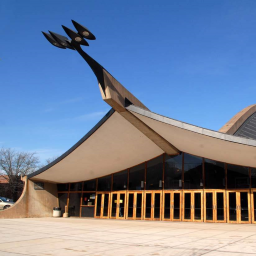
\includegraphics[width=3.25in]{ingalls.png}
\caption{Ingalls hockey rink.}
\label{ingalls}
\end{figure}

\begin{figure}[!t]
\centering
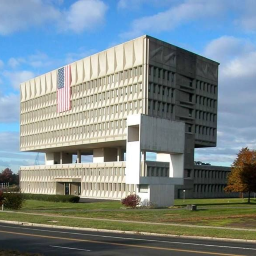
\includegraphics[width=3.25in]{armstrong.png}
\caption{Armstrong building.}
\label{armstrong}
\end{figure}

\begin{figure}[!t]
\centering
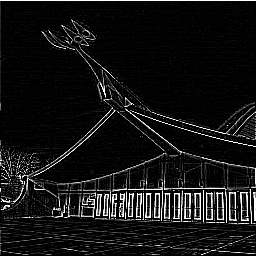
\includegraphics[width=3.25in]{ingalls-high-pass.png}
\caption{Image with high pass filter applied.}
\label{ingalls-high-pass}
\end{figure}

\begin{figure}[!t]
\centering
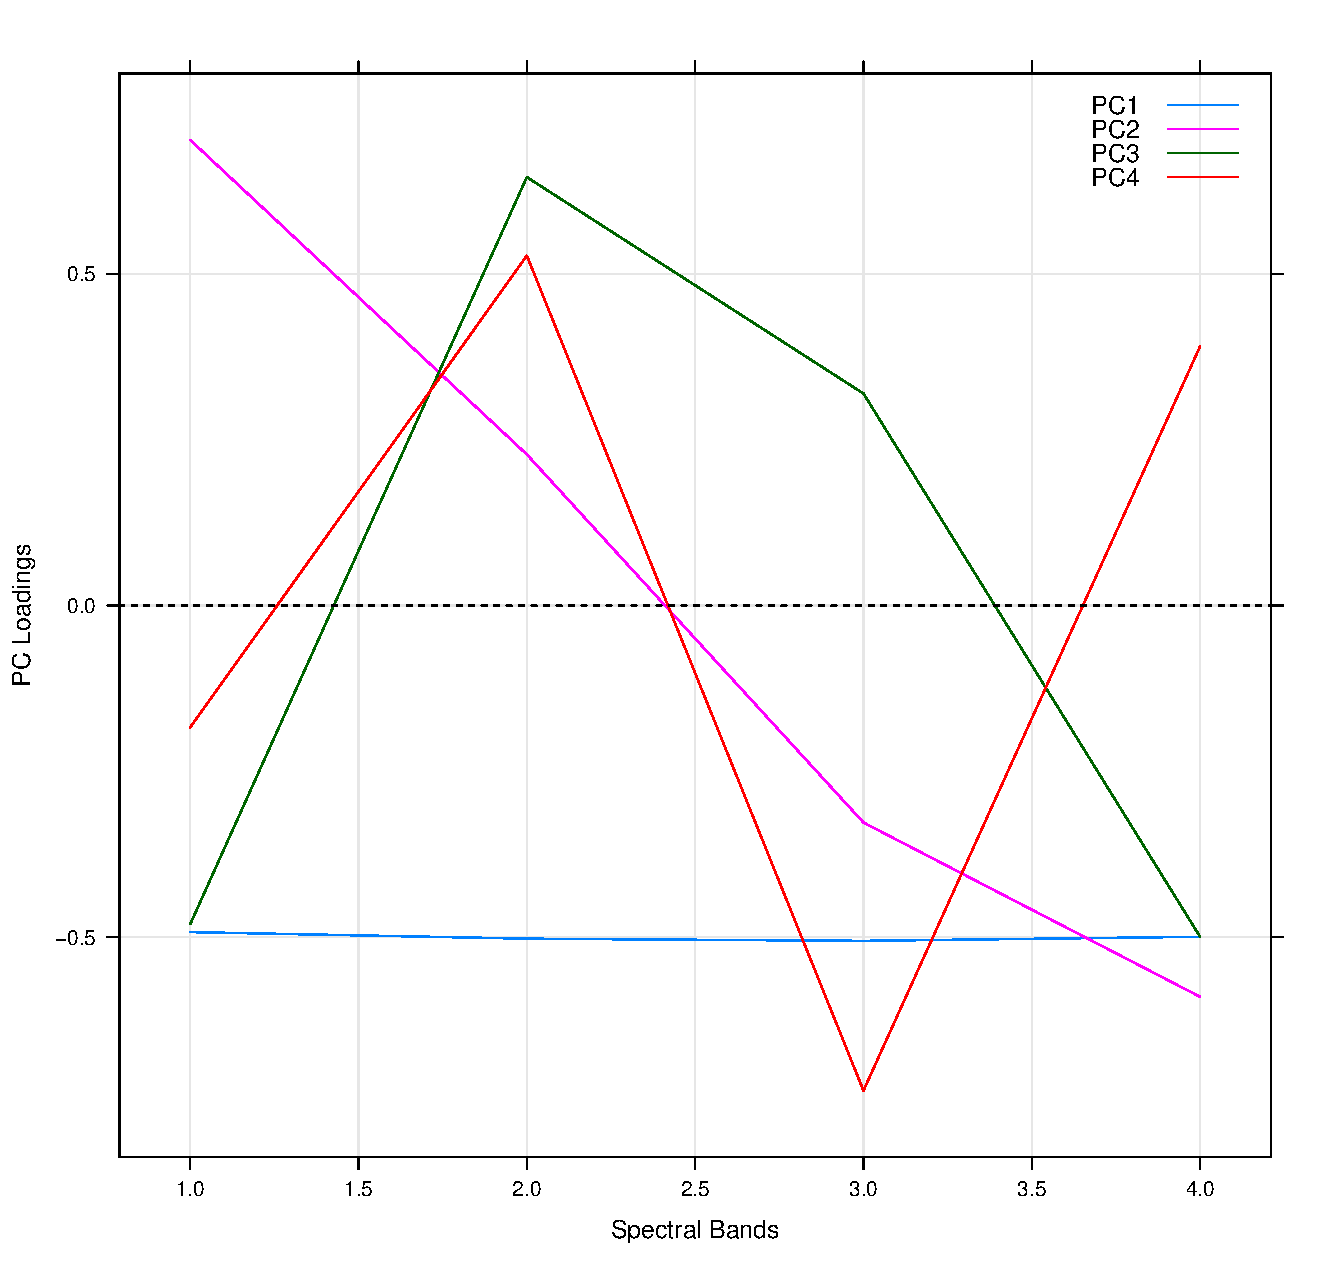
\includegraphics[width=3.25in]{pca-plot.pdf}
% where an .eps filename suffix will be assumed under latex, 
% and a .pdf suffix will be assumed for pdflatex; or what has been declared
% via \DeclareGraphicsExtensions.
\caption{Principal components.}
\label{pca-plot}
\end{figure}

\begin{figure}[!t]
\centering
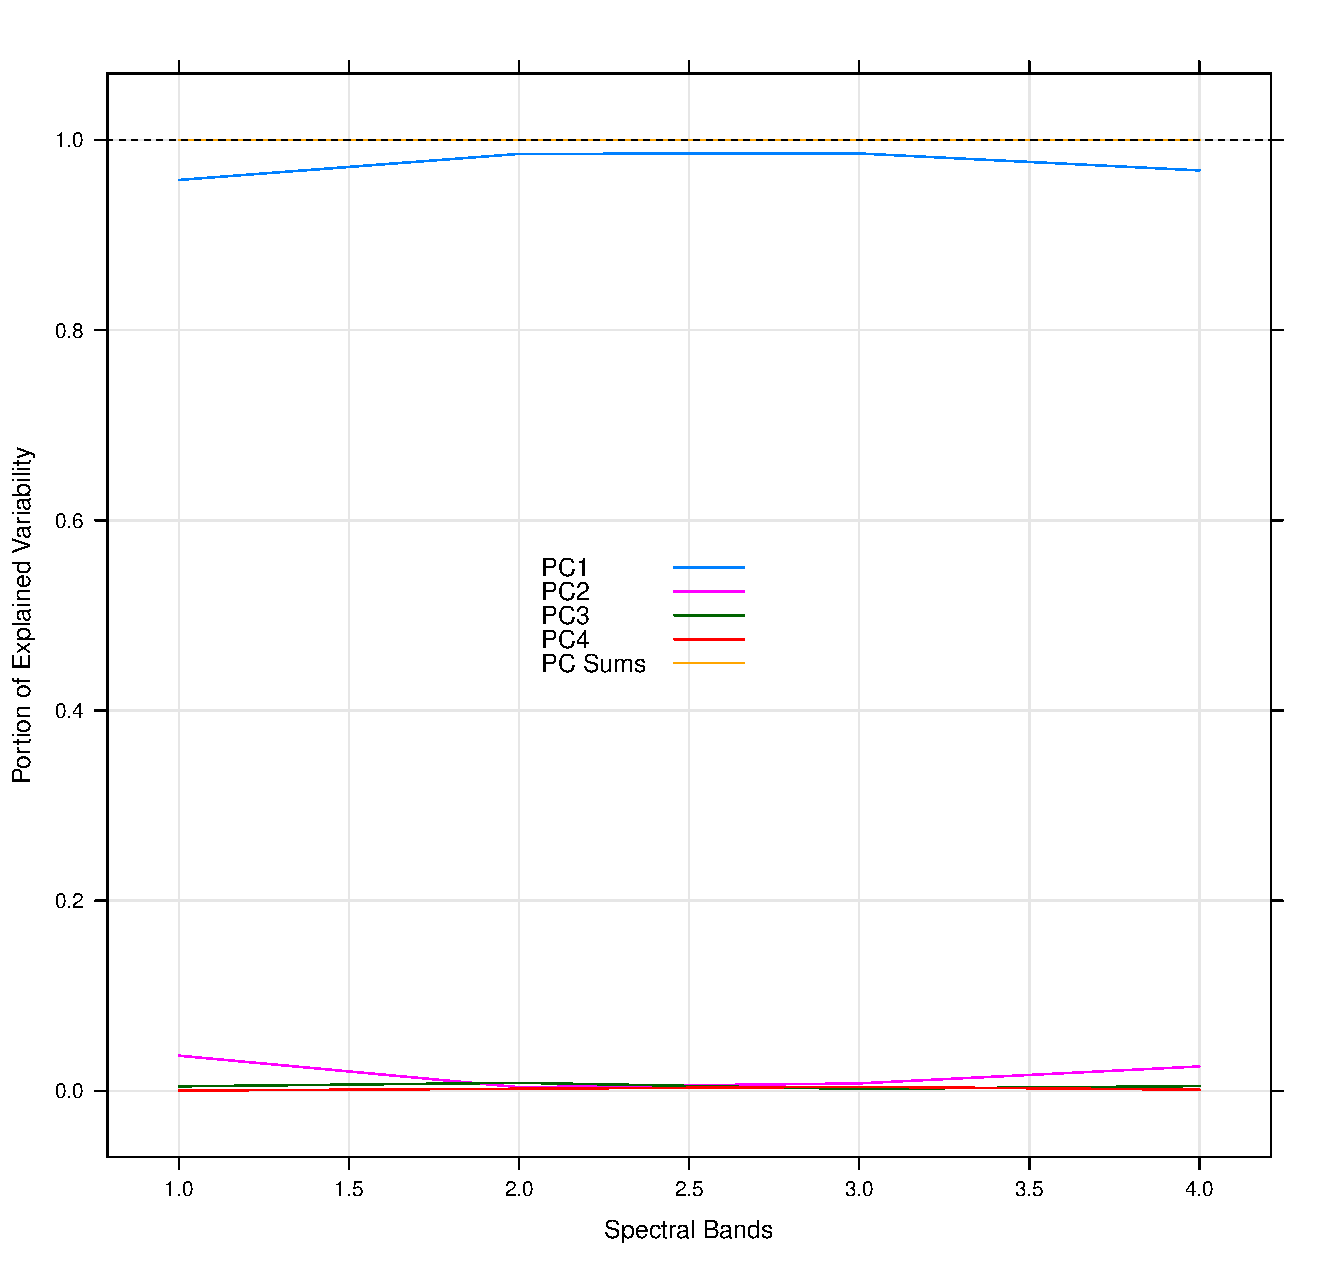
\includegraphics[width=3.25in]{portion-of-variability-plot.pdf}
\caption{Portions of variability.}
\label{portion-of-variability}
\end{figure}

\begin{figure}[!t]
\centering
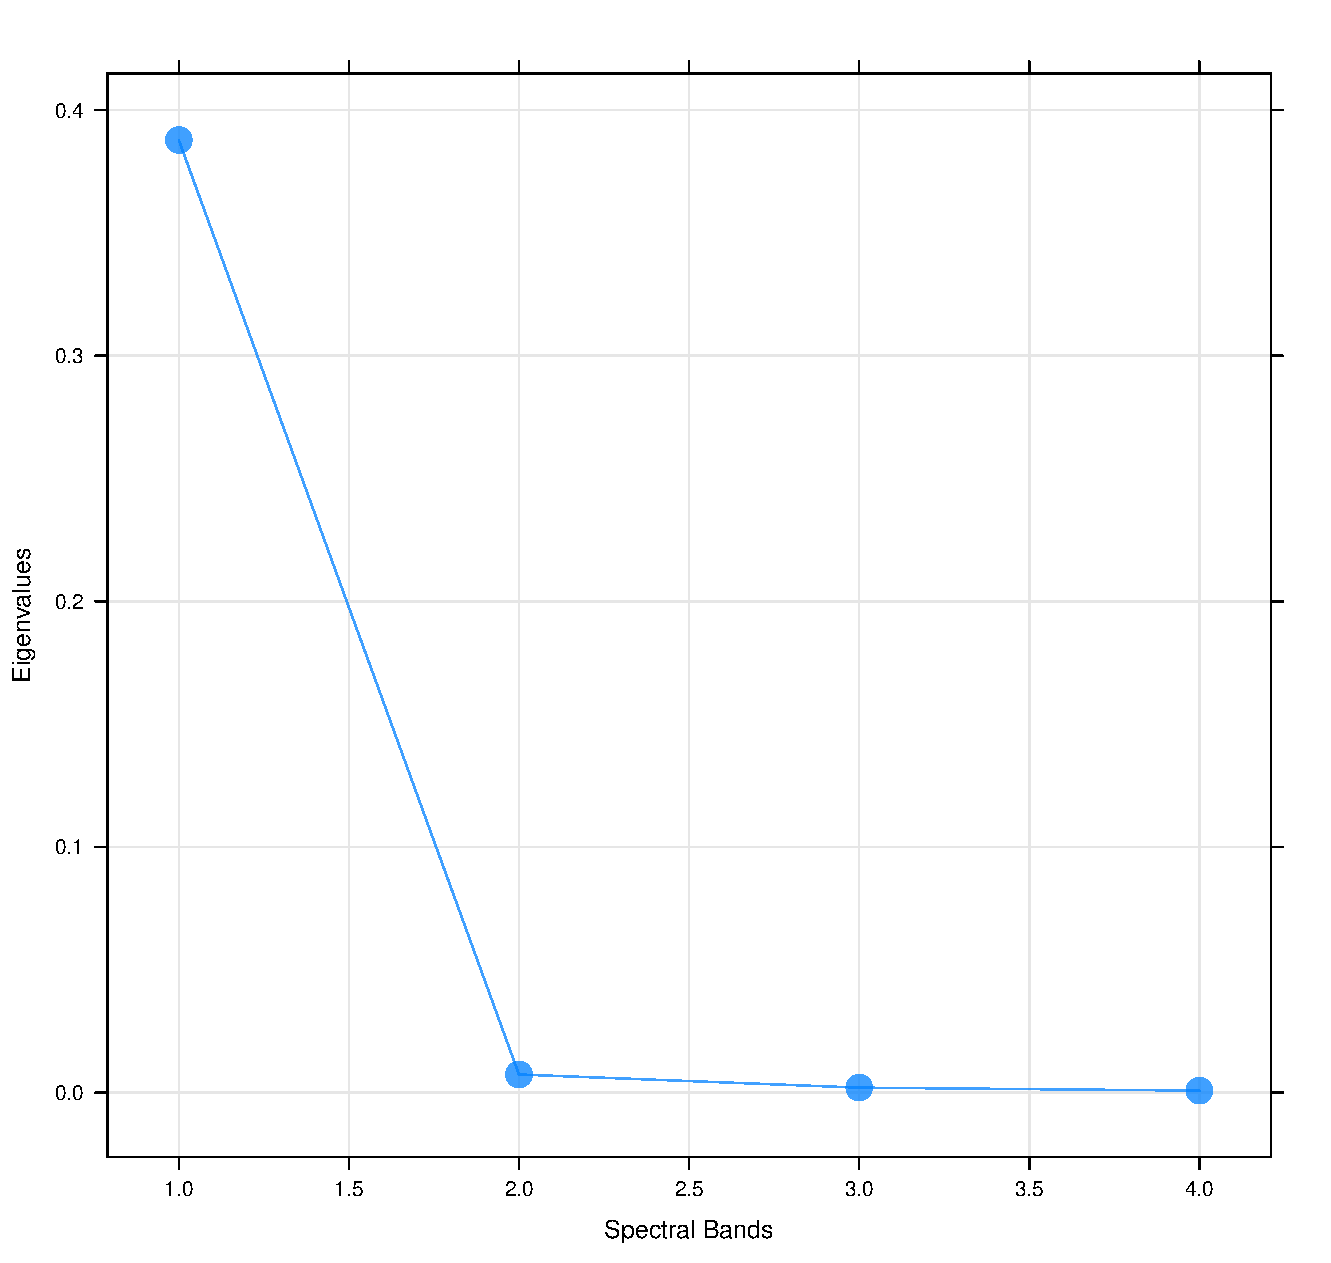
\includegraphics[width=3.25in]{scree-plot.pdf}
\caption{Scree plot.}
\label{scree-plot}
\end{figure}

\begin{figure}[!t]
\centering
\includegraphics[width=3.25in]{pc1.pdf}
\caption{PC1.}
\label{pc1}
\end{figure}

\begin{figure*}[!t]
\centering
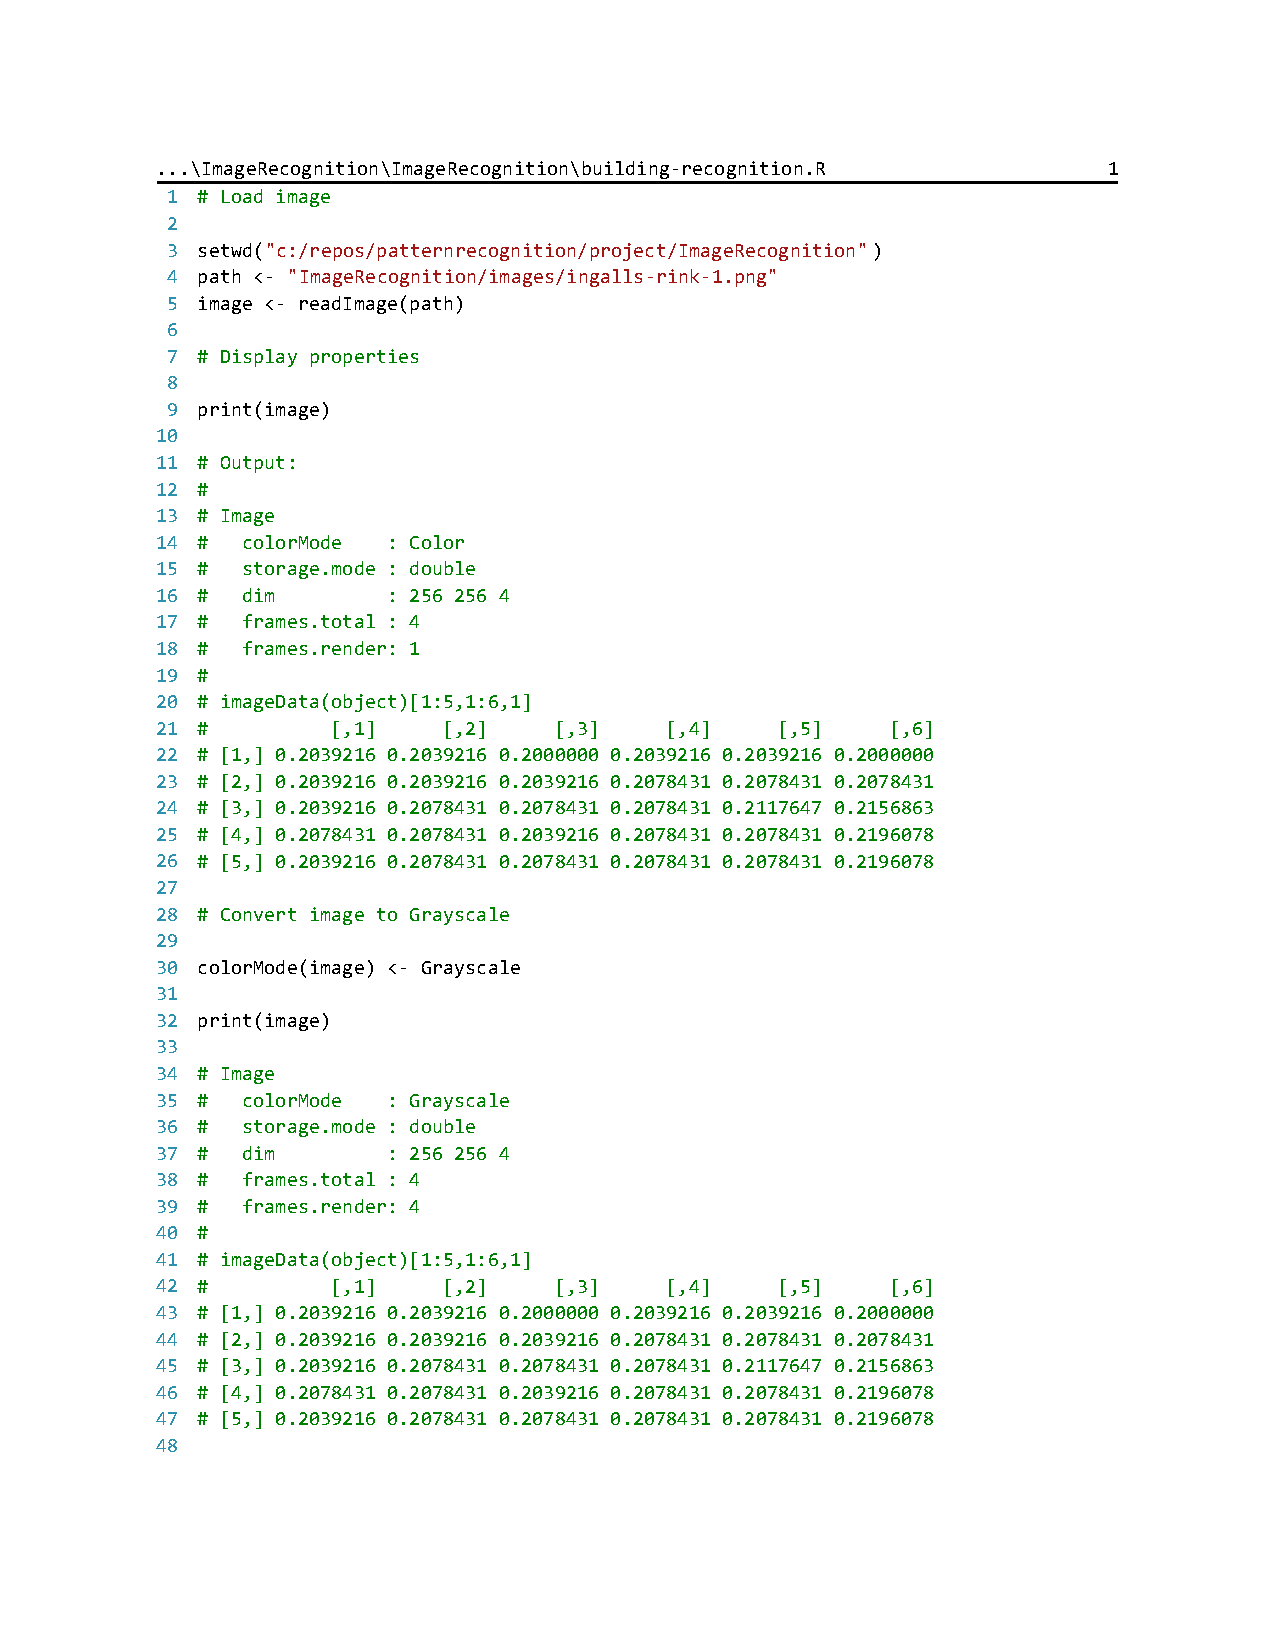
\includegraphics[width=7in]{code-listing-1.pdf}
\caption{Code listing 1.}
\label{code-listing-1}
\end{figure*}

\begin{figure*}[!t]
\centering
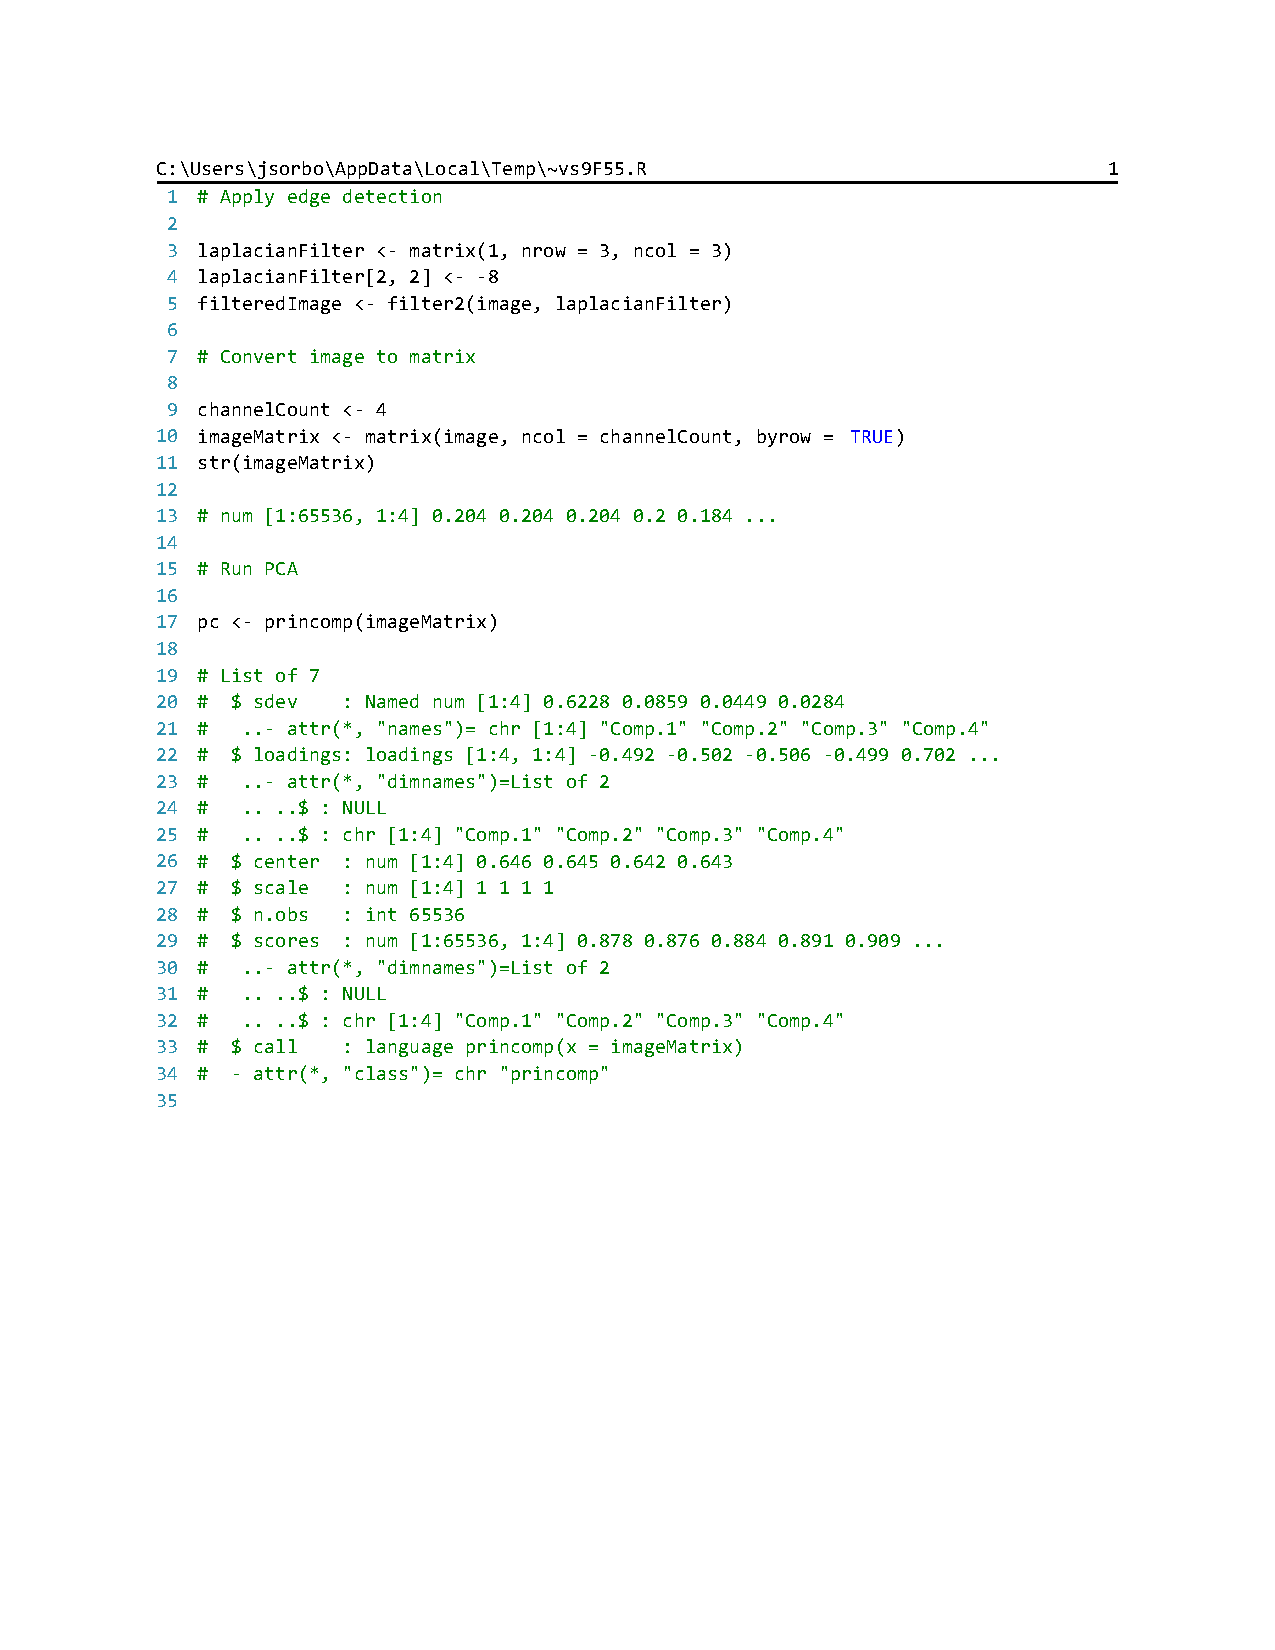
\includegraphics[width=7in]{code-listing-2.pdf}
\caption{Code listing 2.}
\label{code-listing-2}
\end{figure*}

\begin{figure*}[!t]
\centering
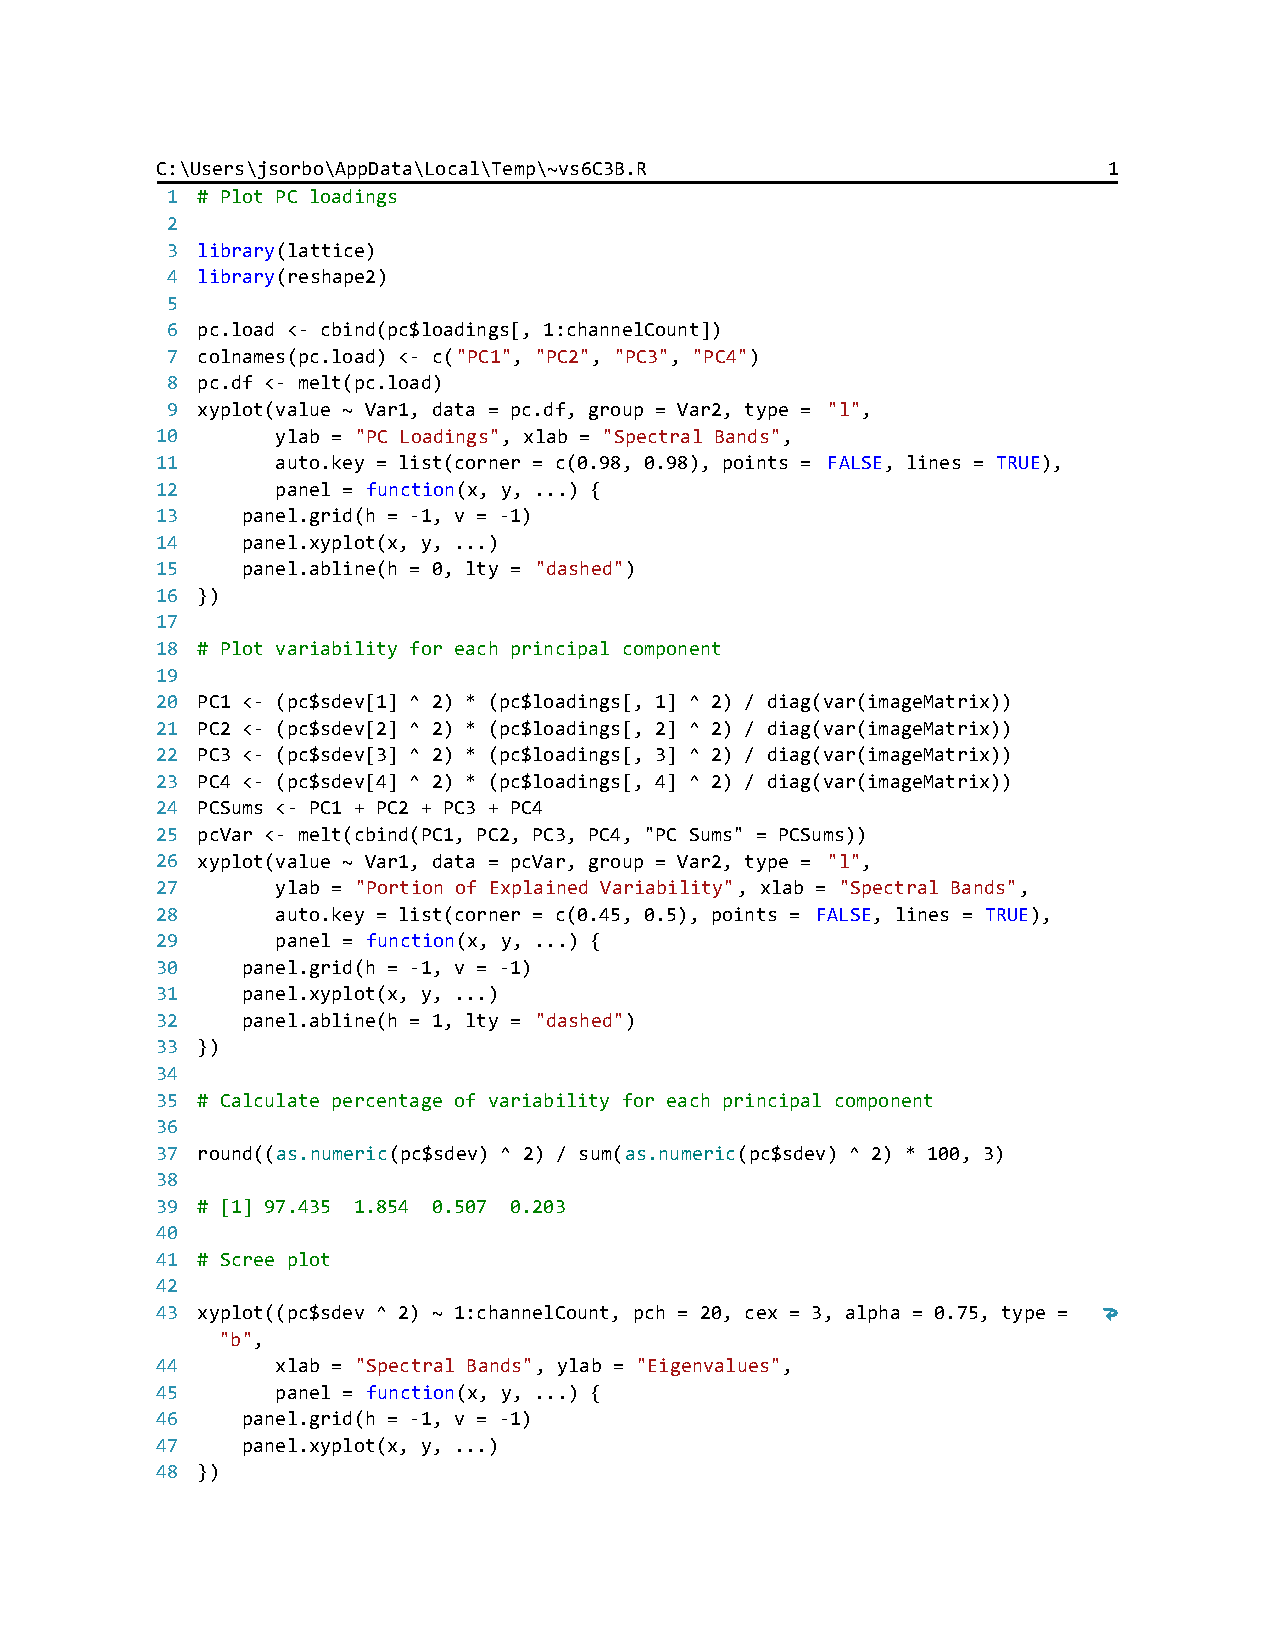
\includegraphics[width=7in]{code-listing-3.pdf}
\caption{Code listing 3.}
\label{code-listing-3}
\end{figure*}

\begin{figure*}[!t]
\centering
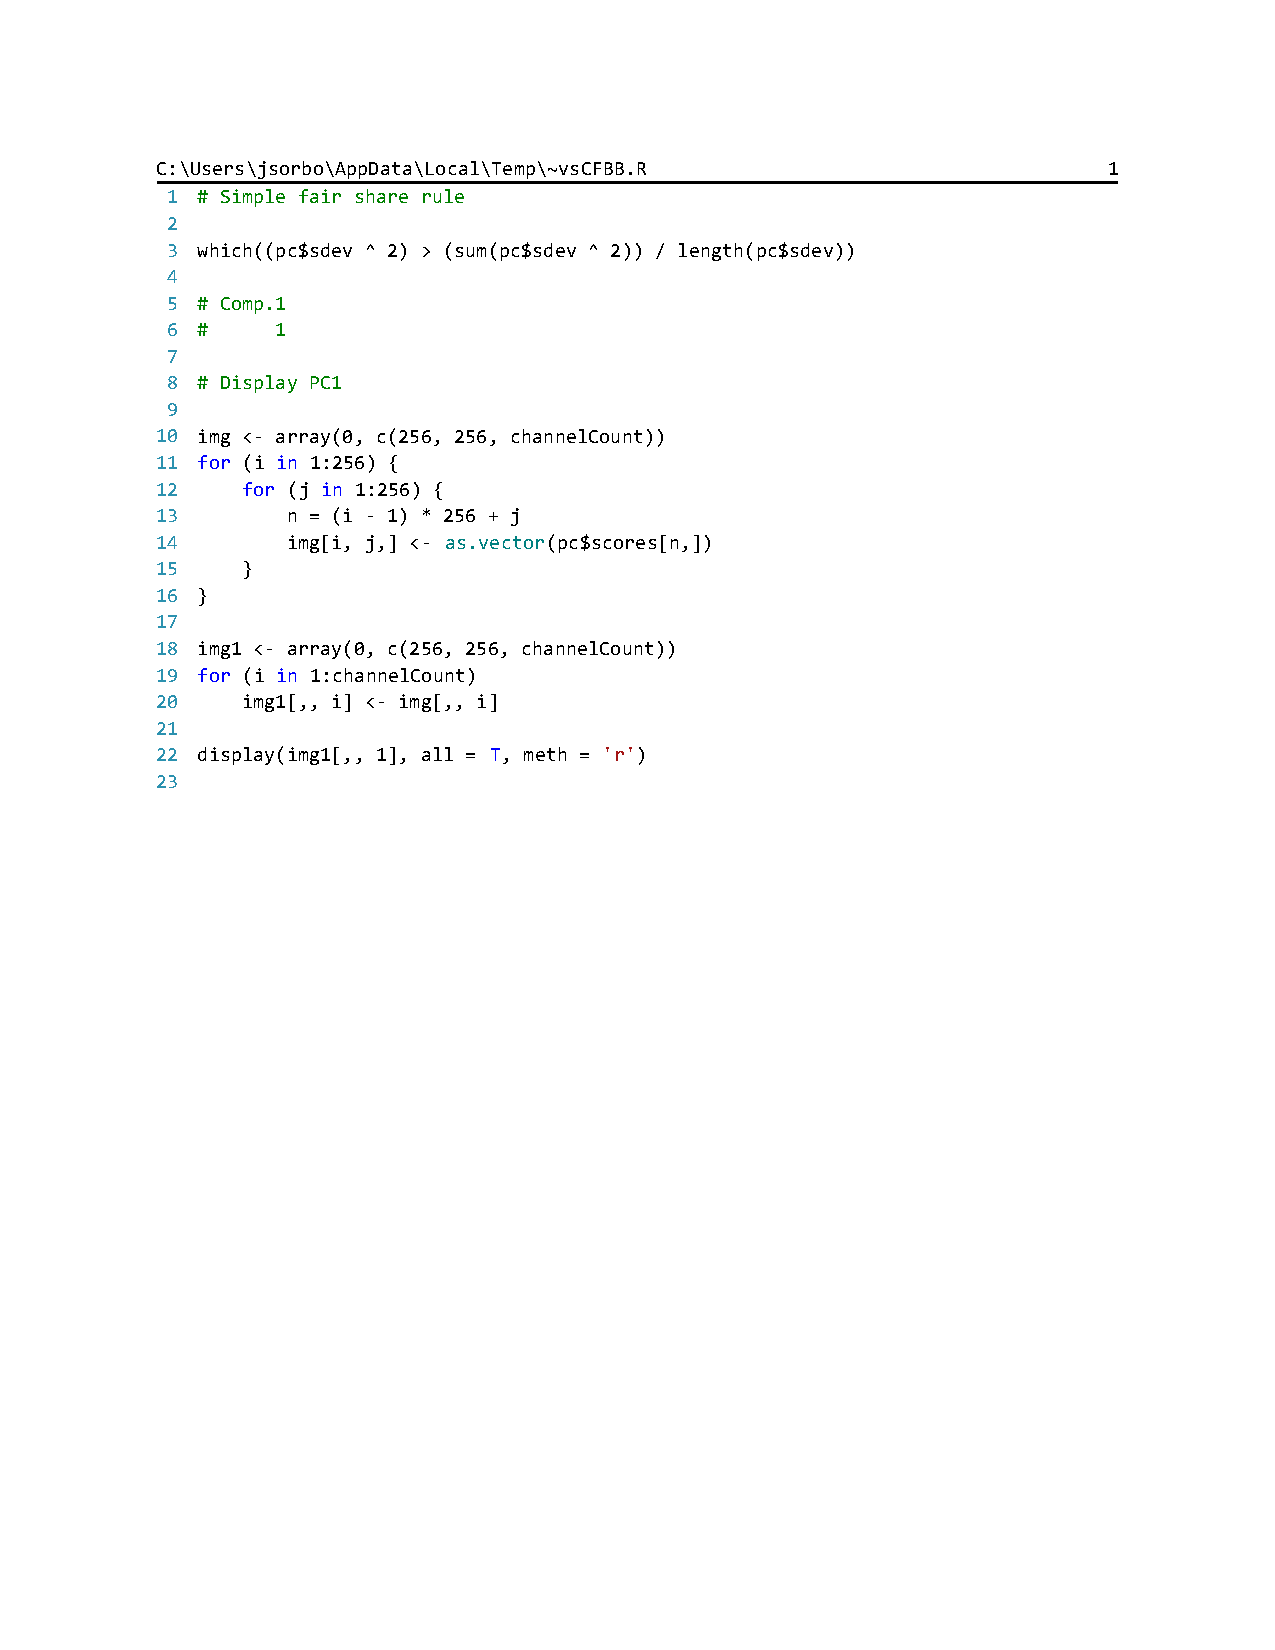
\includegraphics[width=7in]{code-listing-4.pdf}
\caption{Code listing 4.}
\label{code-listing-4}
\end{figure*}

\begin{table}[!t]
% increase table row spacing, adjust to taste
\renewcommand{\arraystretch}{1.3}
% if using array.sty, it might be a good idea to tweak the value of
% \extrarowheight as needed to properly center the text within the cells
\caption{Principal Component Percentages of Variability}
\label{percentages}
\centering
% Some packages, such as MDW tools, offer better commands for making tables
% than the plain LaTeX2e tabular which is used here.
\begin{tabular}{cc}
\hline
Component & Percentage\\
\hline
PC1 & 97.435\%\\
PC2 & 1.854\%\\
PC3 & 0.507\%\\
PC4 & 0.203\%\\
\hline
\end{tabular}
\end{table}
%%% 97.435  1.854  0.507  0.203

% trigger a \newpage just before the given reference
% number - used to balance the columns on the last page
% adjust value as needed - may need to be readjusted if
% the document is modified later
%\IEEEtriggeratref{8}
% The "triggered" command can be changed if desired:
%\IEEEtriggercmd{\enlargethispage{-5in}}

% references section

% can use a bibliography generated by BibTeX as a .bbl file
% BibTeX documentation can be easily obtained at:
% http://mirror.ctan.org/biblio/bibtex/contrib/doc/
% The IEEEtran BibTeX style support page is at:
% http://www.michaelshell.org/tex/ieeetran/bibtex/
%\bibliographystyle{IEEEtran}
% argument is your BibTeX string definitions and bibliography database(s)
%\bibliography{IEEEabrv,../bib/paper}
%
% <OR> manually copy in the resultant .bbl file
% set second argument of \begin to the number of references
% (used to reserve space for the reference number labels box)

% JSS steps to compile latex + biblatex
% 1. pdflatex traffic-classification.tex
% 2. bibtex traffic-classification (will look for .aux extension, do not specify in argument though)
% 3. pdflatex traffic-classification.tex
% 4. pdflatex traffic-classification.tex (again)

\bibliographystyle{ieeetr}
\bibliography{datta,bajorski}

%%%%%% \appendix{Code Listings}
%%%%%% 
%%%%%% \begin{lstlisting}[frame=single]
%%%%%% library("EBImage")
%%%%%% setwd("c:/jsorbo/repos/patternrecognition/project/ImageRecognition")
%%%%%% path <- "ImageRecognition/images/ingalls-rink-1.png"
%%%%%% image<-readImage(path)
%%%%%% 
%%%%%% \end{lstlisting}

\end{document}
